\documentclass[conference]{IEEEtran}
\IEEEoverridecommandlockouts
\usepackage[utf8]{inputenc}
\usepackage[T1]{fontenc}
\usepackage{cite}
\usepackage{amsmath}
\usepackage{graphicx}
\usepackage{booktabs}
\usepackage{xcolor}
\usepackage{url}
\usepackage{tikz}
\usetikzlibrary{arrows.meta,positioning,shapes.geometric}
\graphicspath{{figures/}}
\newcommand{\qwen}{Qwen3.5-0.8B}
\newcommand{\lfm}{LFM2.5-1.2B-Instruct}
\newcommand{\gemma}{Gemma~4 E2B-it}

\begin{document}

\title{A Comparative Evaluation of Quantized Small Language Models on Raspberry Pi 4B: Inference Performance, Resource Usage, and Task Quality}

\author{\IEEEauthorblockN{JoshuaHM-p4}
\IEEEauthorblockA{Independent evaluation\\
}}

\maketitle

\begin{abstract}
Three quantized small language models were deployed with one pinned llama.cpp build on a single Raspberry Pi~4 Model~B (4\,GB RAM, CPU only, stock clocks): \qwen{} (Q4\_K\_M), \lfm{} (Q4\_K\_M), and \gemma{} (Q4\_0). Feasibility, synthetic throughput, resource use, and task quality were measured as separate kinds of evidence under a protocol frozen after a pilot. All three loaded at a 2{,}048-token context; \gemma{} occupied about 2.9\,GB and swapped to compressed RAM on its first load. Generation ran at 5.24, 5.00, and 2.35 tokens/s, respectively. On a 20-prompt personal task suite scored blind for correctness and instruction adherence (0--2 each), \gemma{} scored 38/40 and 39/40, \lfm{} 33/40 and 34/40, and \qwen{} 32/40 and 31/40, while only the two smaller models answered most prompts within a pre-declared 10\,s budget (17/20 each versus 8/20). No throttling or undervoltage occurred. The study recommends \lfm{} as an interactive default and \gemma{} for accuracy-critical requests on this board; all raw logs, answers, and scoring files are published.
\end{abstract}

\begin{IEEEkeywords}
small language models, edge inference, Raspberry Pi, quantization, llama.cpp, benchmarking
\end{IEEEkeywords}

\section{Introduction}
A local text assistant on an inexpensive single-board computer avoids network dependence and keeps data on the device, but only if a model fits in memory, answers quickly enough, and answers correctly. Vendor throughput figures are measured on other hardware~\cite{gemma4overview}, and a quantized file fitting on disk does not imply that inference fits in RAM. This work therefore measures three candidate deployments on the actual target, a 4\,GB Raspberry Pi~4B~\cite{rpidocs}, and keeps three kinds of evidence apart: \emph{feasibility} (does it load and finish), \emph{performance and resources} (how fast, how much memory, what temperatures), and \emph{task quality} (is the answer right and does it follow the request).

The contributions are: (i) a reproducible protocol with a feasibility gate, a pilot, and a frozen measurement phase; (ii) measured throughput, memory, thermal, and answer-time results for three current small models on the same board; (iii) a blinded two-dimensional quality evaluation with executed code tests; and (iv) a public repository with every raw log, answer, and scoring file~\cite{repo}. The results describe these deployments on this board; they do not rank the models in general.

\section{Experimental Setup}

\subsection{Hardware and Runtime}
Table~\ref{tab:setup} lists the platform. The runtime is llama.cpp~\cite{llamacpp} at tag v1.0.0, built natively with only the CPU backend; the build detected a Cortex-A72 without dot-product or int8 matrix extensions. The board runs on a 5\,V\,2\,A supply, below the 5\,V\,3\,A specification~\cite{rpidocs}, so throttle and undervoltage flags were read before and after every session.

\begin{table}[t]
\caption{Platform and Runtime}
\label{tab:setup}
\centering
\footnotesize
\begin{tabular}{@{}ll@{}}
\toprule
Board & Raspberry Pi 4B Rev 1.5, 4\,GB (3796\,MiB usable) \\
OS / kernel & Debian 13 (aarch64), Linux 6.18.50 \\
CPU & 4$\times$ Cortex-A72, 1.8\,GHz stock, \texttt{ondemand} \\
Cooling / power & Heatsink + 5\,V GPIO fan; 5\,V\,2\,A supply \\
Swap & 2\,GiB zram (compressed RAM), unchanged \\
Storage & 32\,GB microSD \\
Runtime & llama.cpp b1b770d (v1.0.0), GCC 14.2, CPU only \\
\bottomrule
\end{tabular}
\end{table}

\subsection{Models}
Table~\ref{tab:models} lists the artifacts, pinned by repository revision and SHA-256~\cite{qwen35gguf,lfm25gguf,gemma4gguf}. Q4\_K\_M was preferred; the official llama.cpp conversion of \gemma{} is only available at Q4\_0 near 4~bits, which is disclosed as a confound. Qwen publishes no official GGUF, so a widely used third-party conversion was used. \gemma{} is an effective-parameter model whose total parameter count (including per-layer embeddings) is much larger than its effective size~\cite{gemma4overview}.

\begin{table}[t]
\caption{Model Artifacts (parameter counts reported by llama-bench)}
\label{tab:models}
\centering
\footnotesize
\begin{tabular}{@{}lrrl@{}}
\toprule
Model & Params & File & Quant. / source \\
\midrule
\qwen{} & 0.75\,B & 533\,MB & Q4\_K\_M / unsloth \\
\lfm{} & 1.17\,B & 731\,MB & Q4\_K\_M / Liquid AI \\
\gemma{} & 4.63\,B$^{\dagger}$ & 2{,}841\,MB & Q4\_0 / ggml-org \\
\bottomrule
\multicolumn{4}{@{}l}{\scriptsize $^{\dagger}$Total stored parameters; ``E2B'' denotes about 2\,B effective.}
\end{tabular}
\end{table}

\subsection{Protocol}
Fig.~\ref{fig:pipeline} shows the protocol. A \emph{feasibility gate} loaded each model in llama-server~\cite{llamaserver} at a 2{,}048-token context and requested one short non-scored answer while sampling memory, swap, temperature, and throttle flags at 1\,Hz. A \emph{pilot} of two non-scored prompts verified that thinking modes were disabled (inspecting every rendered prompt), that the 128-token cap counts generated tokens only, and how long answers take. The prompt set, settings, and a personal acceptable wait of 10\,s were then \emph{frozen} by checksum before any scored answer was collected.

\begin{figure}[t]
\centering
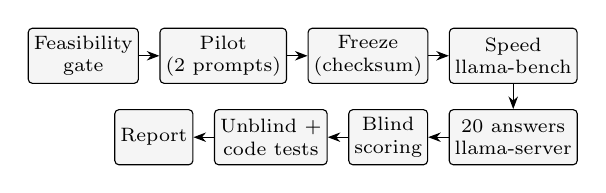
\begin{tikzpicture}[node distance=3.2mm and 2.6mm, font=\scriptsize,
  box/.style={draw, rounded corners=1.5pt, align=center, minimum height=7mm, inner sep=2pt, fill=gray!8},
  arr/.style={-{Stealth[length=1.6mm]}, thin}]
\node[box] (gate) {Feasibility\\gate};
\node[box, right=of gate] (pilot) {Pilot\\(2 prompts)};
\node[box, right=of pilot] (freeze) {Freeze\\(checksum)};
\node[box, right=of freeze] (speed) {Speed\\llama-bench};
\node[box, below=of speed] (quality) {20 answers\\llama-server};
\node[box, left=of quality] (blind) {Blind\\scoring};
\node[box, left=of blind] (unblind) {Unblind +\\code tests};
\node[box, left=of unblind] (report) {Report};
\draw[arr] (gate) -- (pilot); \draw[arr] (pilot) -- (freeze); \draw[arr] (freeze) -- (speed);
\draw[arr] (speed) -- (quality); \draw[arr] (quality) -- (blind); \draw[arr] (blind) -- (unblind);
\draw[arr] (unblind) -- (report);
\end{tikzpicture}
\caption{Evaluation protocol. Each stage writes append-only raw files that are published with the paper.}
\label{fig:pipeline}
\end{figure}

\emph{Speed.} llama-bench~\cite{llamabench} measured prompt processing at 128 and 512 tokens (pp128, pp512) and generation of 64 tokens (tg64) with 4 threads and batch and micro-batch 128: one excluded warm-up, then three repetitions per condition. Sessions ran in the order \qwen{}, \lfm{}, \gemma{}, each starting at or below 45\,$^\circ$C. Peak resident set size (RSS) of the measured process was taken from GNU \texttt{time}.

\emph{Quality.} Twenty original prompts cover five categories (instruction following, extraction and classification, reasoning, summarization, small Python functions), four each. Each prompt was sent as a fresh single-turn chat containing only the prompt text, with the model's native template, greedy decoding (temperature 0), at most 128 generated tokens, thinking disabled through the template's \texttt{enable\_thinking} flag, and prompt caching off. Client-observed, non-streaming answer time was recorded; it includes prompt processing and generation and is not time to first token.

\emph{Scoring.} One scorer graded every answer 0--2 for correctness and 0--2 for adherence against a reference and written criteria, on a sheet that grouped answers by prompt, shuffled models, and hid identities behind random codes. Coding answers were executed against the prompts' test cases in a network-less, read-only container on a separate machine, never on the Pi.

\section{Results}

\subsection{Feasibility}
All three models loaded and completed the gate with a stop finish reason and thinking disabled. \qwen{} and \lfm{} loaded in 2--3\,s with no swap activity. \gemma{} loaded in 80\,s on its first attempt, when the page cache was full from downloading the file, and pushed 56{,}921 pages (about 222\,MB) to zram during loading only; an identical second attempt loaded in 8\,s without swap-out. It is therefore classified as \emph{ready with restrictions}: it fits, but with under 1\,GB of headroom.

\subsection{Throughput and Thermals}
Fig.~\ref{fig:speed} reports llama-bench means and standard deviations; run-to-run variation was below 0.3\%. \qwen{} processed prompts fastest (19.31 tokens/s at pp512) and generated fastest (5.24 tokens/s). \lfm{} generated almost as fast (5.00) but processed prompts more slowly (12.23). \gemma{} processed prompts faster than \lfm{} (14.86) but generated at less than half the speed (2.35). Fig.~\ref{fig:thermal} shows the system-on-chip temperature during the speed sessions: the maximum sampled temperature was 57.0\,$^\circ$C, far below the 80\,$^\circ$C soft-throttle threshold, and no throttle or undervoltage flag was set at any time despite the 2\,A supply.

\begin{figure}[t]
\centering
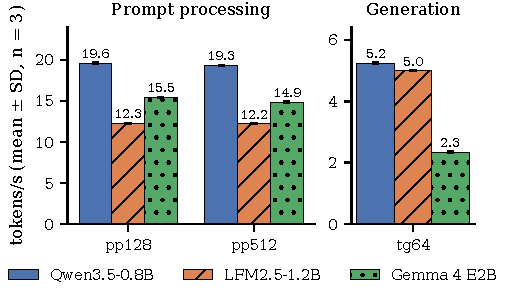
\includegraphics[width=\columnwidth]{speed.pdf}
\caption{llama-bench throughput (mean $\pm$ SD of three repetitions). Error bars are smaller than the line width.}
\label{fig:speed}
\end{figure}

\begin{figure}[t]
\centering
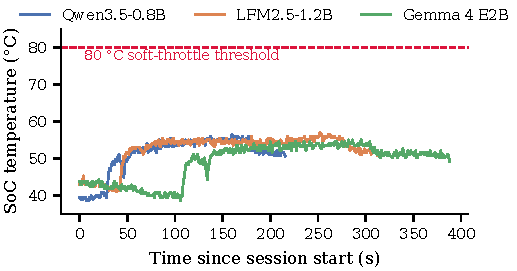
\includegraphics[width=\columnwidth]{thermal.pdf}
\caption{SoC temperature during each speed session (1\,Hz). No throttling occurred.}
\label{fig:thermal}
\end{figure}

\subsection{Memory}
Fig.~\ref{fig:memory} compares the benchmark process's peak RSS with the chat server's peak (VmHWM) during answer collection. Both include memory-mapped weight pages. \gemma{} used about 2.8--2.9\,GB of the 3.8\,GB available. The default llama-server keeps a host-RAM prompt cache that stored each finished request's state even with per-request caching disabled; for \qwen{} this grew the server by about 40\,MB per request to 1.43\,GB. A labelled diagnostic rerun with the cache disabled (\texttt{--cache-ram 0}) peaked at 689\,MB and produced 20/20 byte-identical answers, so the answers are unaffected and deployment sizing should use a capped cache.

\begin{figure}[t]
\centering
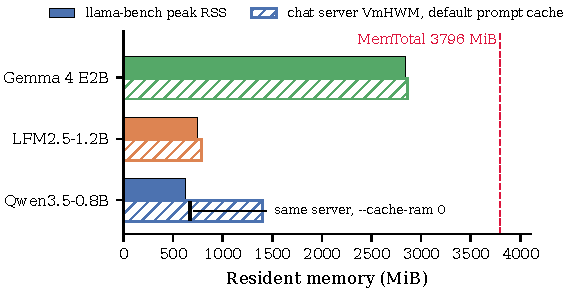
\includegraphics[width=\columnwidth]{memory.pdf}
\caption{Peak resident memory. Hatched bars include llama-server's default prompt cache; the tick on Qwen's bar marks the same server with the cache disabled.}
\label{fig:memory}
\end{figure}

\subsection{Answer Time}
Fig.~\ref{fig:latency} shows the time to a complete answer for each scored prompt. \qwen{} and \lfm{} had nearly identical medians (6.75\,s and 6.72\,s) and answered 17 of 20 prompts within the 10\,s budget. \gemma{} had a median of 10.92\,s, answered 8 of 20 within budget, and took up to 58.6\,s. Each model reached the 128-token cap on exactly one prompt (R04, which invites a step-by-step explanation).

\begin{figure}[t]
\centering
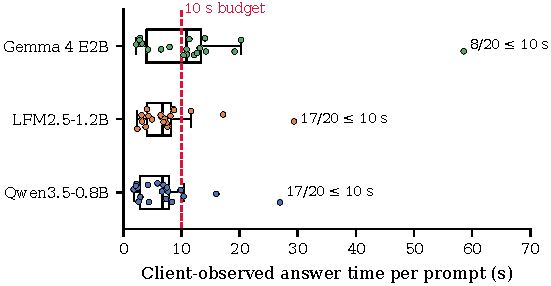
\includegraphics[width=\columnwidth]{latency.pdf}
\caption{Client-observed, non-streaming time per answer for the 20 scored prompts (box: interquartile range; line: median).}
\label{fig:latency}
\end{figure}

\subsection{Task Quality}
Table~\ref{tab:quality} and Fig.~\ref{fig:quality} report scores. All three models were at or near ceiling on instruction following and extraction, and all 27 executed code tests passed for every model. The models differed in reasoning and in honoring explicit constraints. \gemma{} lost points only on R04 (truncated before stating the count) and one omitted summary detail. \lfm{} answered ``9 pens'' to a $12-3+5$ word problem and wrapped two code answers in Markdown fences against instructions. \qwen{} labeled a neutral sentence as positive, used three bullets where exactly two were requested, exceeded a 20-word limit, and introduced an unsupported cause into a summary.

\begin{table}[t]
\caption{Quality Scores (Correctness / Adherence, Maximum 8 per Category)}
\label{tab:quality}
\centering
\footnotesize
\begin{tabular}{@{}lccc@{}}
\toprule
Category & \qwen{} & LFM2.5-1.2B & Gemma 4 E2B \\
\midrule
Instruction & 8 / 8 & 8 / 8 & 8 / 8 \\
Extraction & 6 / 7 & 8 / 8 & 8 / 8 \\
Reasoning & 4 / 5 & 3 / 5 & 7 / 7 \\
Summarization & 6 / 4 & 6 / 7 & 7 / 8 \\
Coding & 8 / 7 & 8 / 6 & 8 / 8 \\
\midrule
Total (/40) & \textbf{32 / 31} & \textbf{33 / 34} & \textbf{38 / 39} \\
Completed / truncated & 19 / 1 & 19 / 1 & 19 / 1 \\
\bottomrule
\end{tabular}
\end{table}

\begin{figure}[t]
\centering
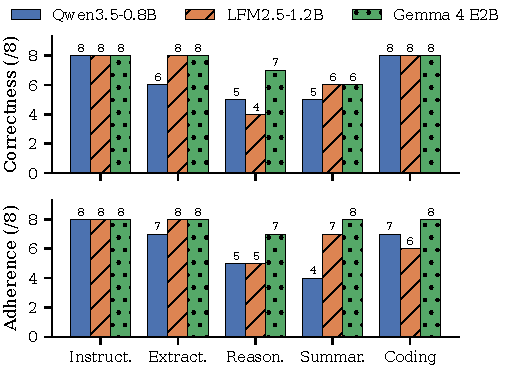
\includegraphics[width=\columnwidth]{quality.pdf}
\caption{Per-category correctness and adherence (blind scoring, all attempts).}
\label{fig:quality}
\end{figure}

\subsection{Trade-off}
Fig.~\ref{fig:tradeoff} combines the three dimensions. The smaller models sit inside the time budget with under 0.8\,GB of memory and similar quality; \gemma{} is clearly more accurate but outside the budget and close to the board's memory limit.

\begin{figure}[t]
\centering
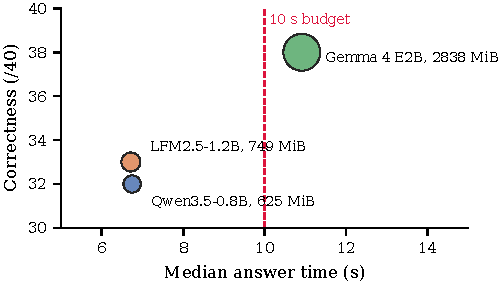
\includegraphics[width=\columnwidth]{tradeoff.pdf}
\caption{Correctness versus median answer time; marker area is proportional to benchmark peak RSS.}
\label{fig:tradeoff}
\end{figure}

\subsection{Greedy Decoding and Repetition}
In the pilot, a request for a 60-item list exposed a failure mode of greedy decoding: \qwen{} repeated three fruits across 25 items, while \lfm{} produced 22 distinct of 26 and \gemma{} 24 of 24 (Fig.~\ref{fig:repetition}). Qwen's model card recommends sampling with a presence penalty in non-thinking mode~\cite{qwen35card}, which motivates the follow-up in Section~\ref{sec:vendor}.

\begin{figure}[t]
\centering
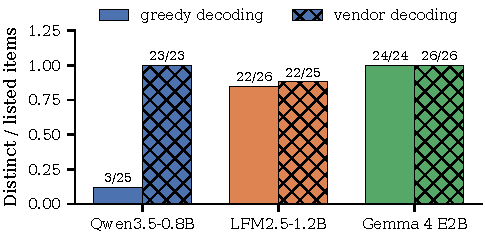
\includegraphics[width=\columnwidth]{repetition.pdf}
\caption{Distinct items in the pilot's 60-fruit list (cut at 128 tokens) under greedy decoding (plain) and vendor-recommended sampling (cross-hatched).}
\label{fig:repetition}
\end{figure}

\section{Follow-up: Vendor-Recommended Sampling}
\label{sec:vendor}
A separately labelled follow-up repeated the pilot and the 20 scored prompts with each vendor's recommended non-thinking sampling~\cite{qwen35card,lfm25card,gemma4card} and a fixed seed (42), one answer per prompt, all other settings unchanged (Table~\ref{tab:vendor}). Parameters a vendor leaves unset were given their neutral values so that llama.cpp's own sampler defaults did not apply.

\begin{table}[t]
\caption{Vendor-Recommended Sampling (Seed 42)}
\label{tab:vendor}
\centering
\footnotesize
\begin{tabular}{@{}lcccc@{}}
\toprule
Model & Temp. & top-$p$ / top-$k$ & Presence & Repeat \\
\midrule
\qwen{} & 1.0 & 1.00 / 20 & 2.0 & 1.00 \\
LFM2.5-1.2B & 0.1 & 1.00 / 50 & 0.0 & 1.05 \\
Gemma 4 E2B & 1.0 & 0.95 / 64 & 0.0 & 1.00 \\
\midrule
\multicolumn{5}{@{}l}{\scriptsize min-$p$ = 0 for all. ``Repeat'' is llama.cpp's repetition penalty.}
\end{tabular}
\end{table}

With its recommended presence penalty, \qwen{} no longer looped: the 60-fruit list contained 23 distinct items out of 23 (Fig.~\ref{fig:repetition}). Sampling also changed behaviour elsewhere: only 9 of \qwen{}'s 20 scored answers were identical to the greedy run (11 for \lfm{}, 10 for \gemma{}), and \qwen{}'s executed code tests fell from 9/9 to 6/9, while both other models kept 9/9. Answer times were essentially unchanged (medians 7.08, 7.06, and 10.88\,s; 18, 18, and 9 answers within 10\,s), as were memory and thermals, and no throttle flag was set. Blinded quality scoring of these 60 answers uses the same rubric and a separate code-to-model key; its scores are recorded in \texttt{data/quality\_scores\_vendor.csv} in the repository~\cite{repo} and are not part of the comparison above.

\section{Discussion and Recommendation}
For a local assistant that should answer short requests within about 10\,s, \qwen{} and \lfm{} are equally fast on this suite and fit comfortably in memory. Their total scores differ by one to three points, which a 20-prompt suite cannot distinguish; they fail differently, with \lfm{} making reasoning errors and \qwen{} missing explicit format constraints and looping under greedy decoding. \gemma{} gives clearly better answers at less than half the generation speed and nearly 3\,GB of memory, which matters on a board that also hosts other services. The personal recommendation is \lfm{} as the interactive default and \gemma{} for non-interactive or accuracy-critical requests. \qwen{} is preferable when inputs are long, since it processes prompts about 1.6$\times$ faster than \lfm{}; its recommended sampling removes the looping but cost three of nine code tests in the follow-up, so its decoding settings should be chosen per task.

\section{Limitations}
The study uses one board, one runtime build, and one quantization per model; Q4\_0 for \gemma{} differs from Q4\_K\_M for the others, and sizes, architectures, and tokenizers differ, so no architectural effect is isolated. Twenty hand-written prompts with one answer each and a single scorer support descriptive, not statistical, comparisons. The first scoring pass was blind; the subsequent separation of correctness from adherence was performed after model identities were shown, although per-model correctness totals were identical in both passes. Greedy decoding is not every vendor's recommended setting, and the 128-token cap penalizes verbose step-by-step answers. Throughput is synthetic, warm, and single-request; answer times are non-streaming. Ambient temperature and electrical energy were not measured.

\section{Conclusion}
On a 4\,GB Raspberry Pi~4B, all three candidates run with llama.cpp on the CPU without throttling. \lfm{} and \qwen{} deliver most short answers within 10\,s in under 0.8\,GB, while \gemma{} gives the best answers at 2.35 tokens/s and about 2.9\,GB. Feasibility, speed, memory, and quality must be read together: the most accurate model is not the most usable one under an interactive time budget on this hardware.

\section*{Data Availability}
Code, the frozen prompt set, every raw log, answer, telemetry file, blind score sheet, and the code-to-model key are available at \url{https://github.com/JoshuaHM-p4/raspi4-slm-benchmark}~\cite{repo}; \texttt{results/SHA256SUMS} records the checksum of every raw and scoring file.

\bibliographystyle{IEEEtran}
\bibliography{references}

\end{document}
